%% abtex2-modelo-trabalho-academico.tex, v-1.7.1 laurocesar
%% Copyright 2012-2013 by abnTeX2 group at http://abntex2.googlecode.com/ 
%%
%% This work may be distributed and/or modified under the
%% conditions of the LaTeX Project Public License, either version 1.3
%% of this license or (at your option) any later version.
%% The latest version of this license is in
%%   http://www.latex-project.org/lppl.txt
%% and version 1.3 or later is part of all distributions of LaTeX
%% version 2005/12/01 or later.
%%
%% This work has the LPPL maintenance status `maintained'.
%% 
%% The Current Maintainer of this work is the abnTeX2 team, led
%% by Lauro César Araujo. Further information are available on 
%% http://abntex2.googlecode.com/
%%
%% This work consists of the files abntex2-modelo-trabalho-academico.tex,
%% abntex2-modelo-include-comandos and abntex2-modelo-references.bib
%%

% ------------------------------------------------------------------------
% ------------------------------------------------------------------------
% abnTeX2: Modelo de Trabalho Academico (tese de doutorado, dissertacao de
% mestrado e trabalhos monograficos em geral) em conformidade com 
% ABNT NBR 14724:2011: Informacao e documentacao - Trabalhos academicos -
% Apresentacao
% ------------------------------------------------------------------------
% ------------------------------------------------------------------------

\documentclass[
	% -- opções da classe memoir --
	12pt,				% tamanho da fonte
	openright,			% capítulos começam em pág ímpar (insere página vazia caso preciso)
	twoside,			% para impressão em verso e anverso. Oposto a oneside
	a4paper,			% tamanho do papel. 
	% -- opções da classe abntex2 --
	%chapter=TITLE,		% títulos de capítulos convertidos em letras maiúsculas
	%section=TITLE,		% títulos de seções convertidos em letras maiúsculas
	%subsection=TITLE,	% títulos de subseções convertidos em letras maiúsculas
	%subsubsection=TITLE,% títulos de subsubseções convertidos em letras maiúsculas
	% -- opções do pacote babel --
	english,			% idioma adicional para hifenização
	brazil,				% o último idioma é o principal do documento
	]{abntex2}


% ---
% PACOTES
% ---

% ---
% Pacotes fundamentais 
% ---
\usepackage{cmap}				% Mapear caracteres especiais no PDF
\usepackage{lmodern}			% Usa a fonte Latin Modern
\usepackage[T1]{fontenc}		% Selecao de codigos de fonte.
\usepackage[utf8]{inputenc}		% Codificacao do documento (conversão automática dos acentos)
\usepackage{lastpage}			% Usado pela Ficha catalográfica
\usepackage{indentfirst}		% Indenta o primeiro parágrafo de cada seção.
\usepackage{color}				% Controle das cores
\usepackage{graphicx}			% Inclusão de gráficos
\usepackage{xspace}
\usepackage{fourier} 
\usepackage{array}
\usepackage{makecell}
\usepackage{graphics}
% ---

% Pacotes extras
\usepackage[table,xcdraw]{xcolor}   % Inclusão de cores em tabelas
\usepackage{todonotes}
\usepackage{multirow}
\usepackage{pdfpages}
% % Abreviações
% \newcommand{\Fw}{\textit{Framework}\xspace}
% \newcommand{\fw}{\textit{framework}\xspace}
% \newcommand{\Fws}{\textit{Frameworks}\xspace}
% \newcommand{\fws}{\textit{frameworks}\xspace}

% \newcommand{\pskel}{{\small \textsf{PSkel}}\xspace}
% \newcommand{\mppa}{{\small \textsf{MPPA-256}}\xspace}

% Acronyms
\usepackage[acronym,nowarn]{glossaries}

\glsdisablehyper

%%%%%%%%%%%%%%%%%%%%%%%%%%%%%%%%%%%%%%%%%%%%%%%%%%%%%%%%%%%%%%%%%%%%
%%% Acronyms list                                                %%%
%%%%%%%%%%%%%%%%%%%%%%%%%%%%%%%%%%%%%%%%%%%%%%%%%%%%%%%%%%%%%%%%%%%%
%%% Importante:                                      
%%% - A lista PRECISA SER MANTIDA ORDENADA
%%%%%%%%%%%%%%%%%%%%%%%%%%%%%%%%%%%%%%%%%%%%%%%%%%%%%%%%%%%%%%%%%%%%

%A
\xnewacronym[amp]{AMP}{Asymmetric Multi-Processing}
\xnewacronym[anova]{ANOVA}{Analysis of Variance}
\xnewacronym[api]{API}{Application Programming Interface}

%B

%C
\xnewacronym[cnoc]{C-NoC}{Control Network-on-Chip}
\xnewacronym[cmp]{CMP}{Chip Multiprocessor}
\xnewacronym[cow]{COW}{Copy-On-Write}
\xnewacronym[cpu]{CPU}{Central Processing Unit}

%D
\xnewacronym[dnoc]{D-NoC}{Data Network-on-Chip}
\xnewacronym[dma][longplural={Direct Memory Accesses}]{DMA}{Direct Memory Access}
\xnewacronym[dram][longplural={Dynamic Random Access Memories}]{DRAM}{Dynamic Random Access Memory}
\xnewacronym[dtlb]{DTLB}{Data Translation Lookaside Buffer}

%E

%F
\xnewacronym[flops]{FLOPS}{\textit{Floating-point Operations per Second}}
\xnewacronym[fos]{FOS}{Factored Operating System}
\xnewacronym[fpga]{FPGA}{Field Programmable Gate Array}

%G
\xnewacronym[gpu]{GPU}{Graphics Processing Unit}

%H
\xnewacronym[hal]{HAL}{Hardware Abstraction Layer}
\xnewacronym[hpc]{HPC}{High-Performance Computing}

%I
\xnewacronym[iid]{i.i.d}{Independent and Identically Distributed}
\xnewacronym[ipc]{IPC}{Inter-Process Communication}
\xnewacronym[isa]{ISA}{Distributed Hash Table}
\xnewacronym[itlb]{ITLB}{Instruction Translation Lookaside Buffer}
\xnewacronym[ieee]{IEEE}{Institute of Electrical and Electronics Engineers}

%J
\xnewacronym[jtlb]{JTLB}{Join Translation Lookaside Buffer}

%K

%L
\xnewacronym[lfour]{L4}{L4 Microkernel}
\xnewacronym[ltlb]{LTLB}{Locked Translation Lookaside Buffer}

%M
\xnewacronym[mimd]{MIMD}{Multiple Instruction Multiple Data}
\xnewacronym[misd]{MISD}{Multiple Instruction Single Data}
\xnewacronym[mmio]{MMIO}{Memory-Mapped I/O}
\xnewacronym[mmu]{MMU}{Memory Management Unit}
\xnewacronym[moosca]{MOOSCA}{Manycore Operating System for Safety-Critical Application}
\xnewacronym[mos]{mOS}{multi Operating System}
\xnewacronym[mpsoc]{MPSoC}{Multiprocessor System-on-Chip}
\xnewacronym[mpu]{MPU}{Memory Protection Unit}

%N
\xnewacronym[noc]{NoC}{Network-on-Chip}
\xnewacronym[norma]{NoRMA}{No Remote Memory Access}
\xnewacronym[nos]{nOS}{Nano-Sized Operating System}
\xnewacronym[numa]{NUMA}{Non-Uniform Memory Access}

%O
\xnewacronym[os]{OS}{Operating System}

%P
\xnewacronym[pe]{PE}{Processing Element}
\xnewacronym[pgas]{PGAS}{Partitioned Global Address Space}
\xnewacronym[pmca]{PMCA}{Programmable Manycore Accelerator}
\xnewacronym[pmio]{PMIO}{Port-Mapped I/O}
\xnewacronym[posix]{POSIX}{Portable Operating System Interface}

%Q
\xnewacronym[qos]{QoS}{Quality of Service}

%R
\xnewacronym[rab]{RAB}{Remapping Address Block}
\xnewacronym[ram][longplural={Random Access Memories}]{RAM}{Random Access Memory}
\xnewacronym[risc]{RISC}{Reduced Instruction Set Computer}
\xnewacronym[rm]{RM}{Resource Manager}
\xnewacronym[rma][longplural={Remote Memory Accesses}]{RMA}{Remote Memory Access}
\xnewacronym[rmem][longplural={Remote Memories}]{RMem}{Remote Memory}

%S
\xnewacronym[simd]{SIMD}{Single Instruction Multiple Data}
\xnewacronym[sisd]{SISD}{Single Instruction Single Data}
\xnewacronym[shm]{SHM}{POSIX Shared Memory}
\xnewacronym[smp]{SMP}{Symmetric Multi-Processing}
\xnewacronym[soc]{SoC}{System-on-a-Chip}
\xnewacronym[spm][longplural={Software-managed Scratchpad Memories}]{SPM}{Software-managed Scratchpad Memory}
\xnewacronym[sram][longplural={Static Random Access Memories}]{SRAM}{Static Random Access Memory}
	
%T
\xnewacronym[tlb]{TLB}{Translation Lookaside Buffer}

%U
\xnewacronym[uma][longplural={Uniform Memory Accesses}]{UMA}{Uniform Memory Access}

%V
\xnewacronym[vliw]{VLIW}{Very Long Instruction Word}

%W
\xnewacronym[watts]{W}{\textit{Watts}}

%%% Local Variables:
%%% mode: latex
%%% TeX-master: "main"
%%% End:

% \makeglossaries
% ---
% Pacotes adicionais, usados apenas no âmbito do Modelo Canônico do abnteX2
% ---
\usepackage{lipsum}				% para geração de dummy text
% ---

% ---
% Pacotes de citações
% ---
%\usepackage[brazilian,hyperpageref]{backref}	 % Paginas com as citações na bibl
\usepackage[alf]{abntex2cite}	                 % Citações padrão ABNT
% --- 
% CONFIGURAÇÕES DE PACOTES
% --- 

% ---
% Configurações do pacote backref
% Usado sem a opção hyperpageref de backref
%\renewcommand{\backrefpagesname}{Citado na(s) página(s):~}
% Texto padrão antes do número das páginas
%\renewcommand{\backref}{}
% Define os textos da citação
%\renewcommand*{\backrefalt}[4]{
%	\ifcase #1 %
%		Nenhuma citação no texto.%
%	\or
%		Citado na página #2.%
%	\else
%		Citado #1 vezes nas páginas #2.%
%	\fi}%
% ---

% ---
% Informações de dados para CAPA e FOLHA DE ROSTO
% ---
\titulo{Desenvolvimento de um Exokernel minimalista para o Processador Manycore MPPA-256}
% \titulo{Desenvolvimento de um Lightweight Exokernel para o Processador Manycore MPPA-256}
\autor{João Vicente Souto}
\local{Florianópolis}
\data{2018}
\orientador{Márcio Bastos Castro}
\coorientador{Pedro Henrique Penna}
\instituicao{%
  Universidade Federal de Santa Catarina
  \par
  Departamento de Informática e Estatística
  \par
  Ciência da Computação}
\tipotrabalho{Trabalho de Conclusão de Curso de Graduação}
% O preambulo deve conter o tipo do trabalho, o objetivo, 
% o nome da instituição e a área de concentração 
\preambulo{Monografia submetida ao Programa
de Graduação em Ciência da Computação
para a obtenção do Grau de Bacharel.}
% ---


% ---
% Configurações de aparência do PDF final

% alterando o aspecto da cor azul
\definecolor{blue}{RGB}{41,5,195}

% informações do PDF
\makeatletter
\hypersetup{
     	%pagebackref=true,
		pdftitle={\@title}, 
		pdfauthor={\@author},
    	pdfsubject={\imprimirpreambulo},
	    pdfcreator={LaTeX with abnTeX2},
		pdfkeywords={abnt}{latex}{abntex}{abntex2}{trabalho acadêmico}, 
		hidelinks,
		colorlinks=false,       	% false: boxed links; true: colored links
    	linkcolor=blue,          	% color of internal links
    	citecolor=blue,        		% color of links to bibliography
    	filecolor=magenta,      	% color of file links
		urlcolor=blue,
		bookmarksdepth=4
}
\makeatother
% --- 

% --- 
% Espaçamentos entre linhas e parágrafos 
% --- 

% O tamanho do parágrafo é dado por:
\setlength{\parindent}{1.3cm}

% Controle do espaçamento entre um parágrafo e outro:
\setlength{\parskip}{0.2cm}  % tente também \onelineskip

% ---
% compila o indice
% ---
\makeindex
% ---

% ----
% Início do documento
% ----
\begin{document}

% Retira espaço extra obsoleto entre as frases.
\frenchspacing 

% ----------------------------------------------------------
% ELEMENTOS PRÉ-TEXTUAIS
% ----------------------------------------------------------
% \pretextual

% ---
% Capa
% ---
\imprimircapa
% ---

% ---
% Folha de rosto
% (o * indica que haverá a ficha bibliográfica)
% ---
\imprimirfolhaderosto*
% ---

% ---
% Inserir a ficha bibliografica
% ---

% Isto é um exemplo de Ficha Catalográfica, ou ``Dados internacionais de
% catalogação-na-publicação''. Você pode utilizar este modelo como referência. 
% Porém, provavelmente a biblioteca da sua universidade lhe fornecerá um PDF
% com a ficha catalográfica definitiva após a defesa do trabalho. Quando estiver
% com o documento, salve-o como PDF no diretório do seu projeto e substitua todo
% o conteúdo de implementação deste arquivo pelo comando abaixo:
%
% % \begin{fichacatalografica}
% %     \includepdf{fig_ficha_catalografica.pdf}
% % \end{fichacatalografica}
% \begin{fichacatalografica}
% 	\vspace*{\fill}					% Posição vertical
% 	\hrule							% Linha horizontal
% 	\begin{center}					% Minipage Centralizado
% 	\begin{minipage}[c]{12.5cm}		% Largura
	
% 	Podestá Junior, Emmanuel
	
% 	\hspace{0.5cm} \imprimirtitulo \ / \imprimirautor;  \imprimirorientadorRotulo~\imprimirorientador; \imprimirlocal, \imprimirdata-
	
% 	\hspace{0.5cm} \pageref{LastPage} p. : il. (algumas color.) ; 30 cm.\\
	
% 	%\hspace{0.5cm} \imprimirorientadorRotulo~\imprimirorientador, Coorientador: Daniel Priori \\
	
% 	\hspace{0.5cm}
% 	\imprimirtipotrabalho \ --\ Universidade Federal de Santa Catarina, Departamento de Informática e Estatística, Ciência da Computação,
% 	\imprimirdata.\\
	
% % 	\hspace{0.5cm} Inclui referências \\
	
% % 	\hspace{0.5cm}
% % 		1. Ciência da Computação.
% % 		2. Inteligência Artificial.
% % 		3. Deep Learning.
% % 		I. Mauro Roisenberg.
% % 		II. Daniel Priori.
% % 		III. Universidade Federal de Santa Catarina.
% % 		IV. Título \\ 			
	
% 	%\hspace{8.75cm} CDU 02:141:005.7\\
	
% 	\end{minipage}
% 	\end{center}
% 	\hrule
% \end{fichacatalografica}
% ---

% ---
% Inserir folha de aprovação
% ---

% Isto é um exemplo de Folha de aprovação, elemento obrigatório da NBR
% 14724/2011 (seção 4.2.1.3). Você pode utilizar este modelo até a aprovação
% do trabalho. Após isso, substitua todo o conteúdo deste arquivo por uma
% imagem da página assinada pela banca com o comando abaixo:
%
% \includepdf{folhadeaprovacao_final.pdf}
%
\begin{folhadeaprovacao}

%  \begin{center}
%    {\ABNTEXchapterfont\bfseries\Large FOLHA DE APROVAÇÃO DE PROPOSTA DO TCC}
%    %\hspace{.45\textwidth}
%    %\begin{minipage}{.5\textwidth}
%        %\imprimirpreambulo
%    %\end{minipage}
%    %\vspace*{\fill}
%   \end{center}
%   \renewcommand\theadalign{cb}
%   \renewcommand\theadfont{\bfseries}
%	\renewcommand\theadgape{\Gape[4pt]}
%	\renewcommand\cellgape{\Gape[4pt]}
%   %\def\arraystretch{2}%  1 is the default, change whatever you need
%	\begin{flushleft}
%    \resizebox{\columnwidth}{!}{%
%	\begin{tabular}{|l|l|}
%	\hline
%			\textbf{Acadêmico(s)} &  João Vicente Souto \hspace{74mm} \\ \hline
%            \textbf{Título do Trabalho}  & \makecell[l]{PSkel-MPPA: Uma Adaptação do Framework PSkel para \\ o Processador Manycore %MPPA-256}\\ \hline
%            \textbf{Curso} & Ciências da Computação/INE/UFSC \\ \hline
%            \textbf{Área de Concentração} & \textbf{DETERMINAR ÁREAS DE CONCENTRAÇÃO} \\ \hline
%    \end{tabular}
%    }
%    \end{flushleft}
%    \begin {flushleft}
%    \textbf{Instruções para preenchimento pelo \emph{ORIENTADOR DO TRABALHO}:}
%    \begin{itemize}
%    \item Para cada critério avaliado, assinale um X na coluna SIM apenas se considerado aprovado. Caso contrário, indique as alterações %necessárias na coluna de Observação.
%    \end{itemize}
%    \end{flushleft}
%    \newcolumntype{C}{>{\centering\arraybackslash}p{25em}}
%    \newcolumntype{A}{>{\centering\arraybackslash}p{4em}}
%    \newcolumntype{O}{>{\centering\arraybackslash}p{11em}}
%    \begin{flushleft}
%    \resizebox{\columnwidth}{!}{%
%    \begin{tabular}{|C|A|A|A|A|O|}
%    \hline
%    	\multirow{2}{*}{\textbf{Critérios}} & \multicolumn{4}{c|}{\textbf{Aprovado}} & \multirow{2}{*}{\textbf{Observação}} \\[1ex]
%	\cline{2-5}
%        & \textbf{Sim} & \textbf{Parcial} & \textbf{Não} & \textbf{Não se aplica} & \\
%        \hline
%        \makecell[l]{O trabalho é adequado para um TCC em CCO \\ (relevância / abrangência)?}& & & & & \\
%        \hline
%        \makecell[l]{O título é adequado?}& & & & & \\
%        \hline
%        \makecell[l]{O Tema de pesquisa está claramente descrito?}& & & & & \\
%        \hline
%        \makecell[l]{O problema/hipóteses de pesquisa do trabalho está \\ claramente identificado?}& & & & & \\
%        \hline
%        \makecell[l]{A relevância da pesquisa é justificada?}& & & & & \\
%        \hline
%        \makecell[l]{Os objetivos descrevem completa e claramente o \\ que se pretende alcançar neste trabalho?}& & & & & \\
%        \hline
%        \makecell[l]{É definido o método a ser adotado no trabalho? \\ O método condiz com os objetivos e é adequado \\ para um TCC?}& & %& & & \\
%        \hline
%        \makecell[l]{Foi definido um cronograma coerente com o método\\ definido (indicando todas as atividades) e com as \\ datas das %entregas (p.ex. Projeto I, II, Defesa)?}& & & & & \\
%        \hline
%        \makecell[l]{Foram identificados custos relativos à execução deste \\ trabalho (se houver)? Haverá financiamento para \\ estes %custos?}& & & & & \\
%        \hline
%        \makecell[l]{Foram identificados todos os envolvidos neste \\ trabalho?}& & & & & \\
%        \hline
%        \makecell[l]{As formas de comunicação foram definidas?}& & & & & \\[1ex]
%        \hline
%        \makecell[l]{Riscos potenciais que podem causar desvios do plano \\ foram identificados?}& & & & & \\
%        \hline
%        \makecell[l]{Caso o TCC envolva a produção de um software ou \\ outro tipo de produto e seja desenvolvido também \\ como uma %atividade realizada numa empresa ou \\ laboratório, consta na proposta uma declaração\\ (Anexo 3) de ciência e concordância com a %entrega\\ do código fonte e/ou documentação produzidos?}& & & & & \\
%        \hline
%    \end{tabular}
%    }
%    \newcolumntype{B}{>{\centering\arraybackslash}p{41.72em}}
%    \newcolumntype{E}{>{\centering\arraybackslash}p{7em}}
%    \newcommand\answerbox{%%
%    \fbox{\rule{0.0001ex}{1pt}\rule[0.1ex]{0pt}{0.0001ex}}\hspace{2mm}}
%    \begin{tabular}{|B|}
%    \hline
%    \makecell[l]{Avaliação}\hspace{35mm} \makecell[c]{\answerbox Aprovado \hspace{15mm} \answerbox Não Aprovado} \\ \hline
%    \end{tabular}
%   	\begin{tabular}{|A|A|A|A|}
%    \hline
%    	Professor Responsável & & & \\ \hline
%    \end{tabular}

%    \end{flushleft}
    
   %\imprimirlocal, 13 de junho de 2018:

   %\assinatura{\textbf{Professor} \\ Coordenador do Curso}

   %\textbf{Banca Examinadora:}
   %\assinatura{\textbf{\imprimirorientador} \\ Orientador} 
   %\assinatura{\textbf{Laércio Lima Pilla}}
   %\assinatura{\textbf{Mario Antônio Ribeiro Dantas}}
%    \assinatura{\textbf{Professor}}

%  ******
Critérios de aceitação
% 	\includepdf{Template_Proposta_TCC_V6}

   %\begin{center}
   % \vspace*{0.5cm}
   % {\large\imprimirlocal}
   % \par
   % {\large\imprimirdata}
   % \vspace*{1cm}
  %\end{center}
  
\end{folhadeaprovacao}
% ---

% ---
% Dedicatória
% ---
% \begin{dedicatoria}
%    \vspace*{\fill}
%    \centering
%    \noindent
%    \textit{ Este trabalho é dedicado às crianças adultas que,\\
%    quando pequenas, sonharam em se tornar cientistas.} \vspace*{\fill}
% \end{dedicatoria}
% ---

% ---
% Agradecimentos
% ---
% \begin{agradecimentos}
% Os agradecimentos principais são direcionados à Gerald Weber, Miguel Frasson,
% Leslie H. Watter, Bruno Parente Lima, Flávio de Vasconcellos Corrêa, Otavio Real
% Salvador, Renato Machnievscz\footnote{Os nomes dos integrantes do primeiro
% projeto abn\TeX\ foram extraídos de
% \url{http://codigolivre.org.br/projects/abntex/}} e todos aqueles que
% contribuíram para que a produção de trabalhos acadêmicos conforme
% as normas ABNT com \LaTeX\ fosse possível.

% Agradecimentos especiais são direcionados ao Centro de Pesquisa em Arquitetura
% da Informação\footnote{\url{http://www.cpai.unb.br/}} da Universidade de
% Brasília (CPAI), ao grupo de usuários
% \emph{latex-br}\footnote{\url{http://groups.google.com/group/latex-br}} e aos
% novos voluntários do grupo
% \emph{\abnTeX}\footnote{\url{http://groups.google.com/group/abntex2} e
% \url{http://abntex2.googlecode.com/}}~que contribuíram e que ainda
% contribuirão para a evolução do \abnTeX.

% Os agradecimentos

% \end{agradecimentos}
% ---

% ---
% Epígrafe
% ---
%\begin{epigrafe}
%   \vspace*{\fill}
%	\begin{flushright}
%		\textit{``Não vos amoldeis às estruturas deste mundo, \\
%		mas transformai-vos pela renovação da mente, \\
%		a fim de distinguir qual é a vontade de Deus: \\
%		o que é bom, o que Lhe é agradável, o que é perfeito.\\
%		(Bíblia Sagrada, Romanos 12, 2)}
%	\end{flushright}
%\end{epigrafe}
% ---

% ---
% RESUMOS
% ---

% resumo em português
\begin{resumo}

Ainda precisa ser desenvolvido.

% Aplicações paralelas podem ser classificadas de acordo com o padrão de computação e coordenação. Dentre os padrões mais conhecidos destacam-se o \textit{map}, \textit{reduce}, \textit{pipeline}, \textit{scan} e \textit{stencil}. Este último é muito utilizado em áreas como simulação de física partículas, previsão meteorológica, termodinâmica, resolução de funções diferenciais, manipulação de imagens, entre outras. O PSkel é um \textit{framework} de programação paralela desenvolvido para simplificar o desenvolvimento de aplicações que seguem esse padrão. Utilizando uma abstração de alto nível, o programador define o \emph{kernel} da computação, enquanto o \textit{framework} se encarrega de executar a computação paralela em \textit{multicores} e \textit{Graphics Processing Units} (GPUs) de maneira eficiente.

% O objetivo deste trabalho é propor uma adaptação do \textit{framework} PSkel para o processador \textit{manycore} emergente MPPA-256 batizada de PSkel-MPPA. A motivação para tal adaptação está relacionada à dificuldade de desenvolvimento de aplicações do padrão \textit{stencil} para o MPPA-256, tendo em vista as suas características arquiteturais intrínsecas que tornam o desenvolvimento de aplicações onerosas e suscetíveis a erros. Dentre as principais características destacam-se a sua arquitetura de memória híbrida (memória compartilha e distribuída), comunicação explícita entre processos e ausência de coerência em \textit{cache}. A adaptação do \textit{framework} permitirá simplificar o desenvolvimento de aplicações \textit{stencil} para o MPPA-256, escondendo do desenvolvedor detalhes de implementação tais como a comunicação e a distribuição de computações entre os núcleos de processamento, abstraindo as características que dificultam o desenvolvimento. 

% Serão efetuados diversos experimentos com a solução proposta para o MPPA-256 (PSkel-MPPA) e também em outras arquiteturas suportadas pelo PSkel (\textit{multicores} e GPUs). Esses resultados permitirão a realização de um estudo comparativo dos resultados obtidos. Como métricas, serão considerados o desempenho e a eficiência energética obtidos nessas arquiteturas, além de outras possíveis métricas que possam ser interessantes para o projeto.

%  Segundo a \citeonline[3.1-3.2]{NBR6028:2003}, o resumo deve ressaltar o
%  objetivo, o método, os resultados e as conclusões do documento. A ordem e a extensão
%  destes itens dependem do tipo de resumo (informativo ou indicativo) e do
%  tratamento que cada item recebe no documento original. O resumo deve ser
%  precedido da referência do documento, com exceção do resumo inserido no
%  próprio documento. (\ldots) As palavras-chave devem figurar logo abaixo do
%  resumo, antecedidas da expressão Palavras-chave:, separadas entre si por
%  ponto e finalizadas também por ponto.\citeonline{Emma}.\citeonline{Nielsen}.
%  \citeonline{Goodfellow-et-al-2016}

 \vspace{\onelineskip}
    
 \noindent
 \textbf{Palavras-chaves}: \textit{manycores}. MPPA-256. \textit{exokernel}. \textit{lightweith}.
\end{resumo}

% resumo em inglês
% \begin{resumo}[Abstract]
%  \begin{otherlanguage*}{english}
%    This is the english abstract.

%    \vspace{\onelineskip}
 
%    \noindent 
%    \textbf{Key-words}: latex. abntex. text editoration.
%  \end{otherlanguage*}
% \end{resumo}

% ---
% inserir lista de ilustrações
% ---
%\pdfbookmark[0]{\listfigurename}{lof}
%\listoffigures*
%\cleardoublepage
% ---

% ---
% inserir lista de tabelas
% ---
%\pdfbookmark[0]{\listtablename}{lot}
%\listoftables*
%\cleardoublepage
% ---

% ---
% inserir lista de abreviaturas e siglas
% ---
%\begin{siglas}
%  \item[Fig.] Area of the $i^{th}$ component
%  \item[456] Isto é um número
%  \item[123] Isto é outro número
%  \item[lauro cesar] este é o meu nome
%\end{siglas}
% ---

% ---
% inserir lista de símbolos
% ---
%\begin{simbolos}
%  \item[$ \Gamma $] Letra grega Gama
%  \item[$ \Lambda $] Lambda
%  \item[$ \zeta $] Letra grega minúscula zeta
%  \item[$ \in $] Pertence
%\end{simbolos}
% ---

% ---
% inserir o sumario
% ---
\pdfbookmark[0]{\contentsname}{toc}
\tableofcontents*
\cleardoublepage
% ---



% ----------------------------------------------------------
% ELEMENTOS TEXTUAIS
% ----------------------------------------------------------
\textual


% ----------------------------------------------------------
% Introdução
% ----------------------------------------------------------
\chapter{Projeto}
\section{Introdução}

% An Overview on the Manycore Era
% Nos últimos anos, o aumento constante da frequência de \textit{clock} e aperfeiçoamento de técnicas de paralelismo à nível de instrução deu lugar à corrida pelo aumento do paralelismo à nível de \textit{threads}, dando origem a \textit{chips} com um quantidade elevada de núcleos de processamento, nomeados \textit{multi-core} \cite{overview_hpc}. Porém, como apontado pelo DARPA \cite{DARPA}, o desenvolvimento de plataformas de \hpc mostram aumento exponencial de performance mas também de consumo de energia.

% Durante a década passada, o desempenho de plataformas de Computação de Alto Desempenho (\textit{High Performance Computing} -- HPC) pôde ser atribuído ao crescente número de núcleos de processamento em um único \textit{chip}.
% Porém, o aumento do consumo energético, em paralelo ao aumento da complexidade arquitetural, desses \textit{chips} abriu lugar para pesquisas sobre uma nova categoria de processadores de alto desempenho e baixo consumo energético.

% Um processador que pertença a essa categoria é denominado \textit{low-power manycore processor?} e apresentam diversas características arquitetônicas únicas em comparação aos processadores \textit{multi-cores} existentes \cite{PENNA}, tais como,
% (i) integração de centenas, até milhares, de núcleos em um único Chip,
% (ii) apresentam um sistema de memória restrito e
% (iii) realizam a comunicação por troca de mensagens encima de uma Rede-em-Chip (\textit{Network-On-Chip} -- NoC).
% Desta forma, apesar


% % An Overview on the Manycore Era
% Nos últimos anos, o aumento constante da frequência de \textit{clock} e aperfeiçoamento de técnicas de paralelismo à nível de instrução deu lugar à corrida pelo aumento do paralelismo à nível de \textit{threads}, dando origem a \textit{chips} com um quantidade elevada de núcleos de processamento, nomeados \textit{multi-core} \cite{overview_hpc}. Porém, como apontado pelo DARPA \cite{DARPA}, o desenvolvimento de plataformas de \hpc mostram aumento exponencial de performance mas também de consumo de energia.


% ==================== 1 =======================
% An Overview on the Manycore Era
Nas últimas décadas, a medida que os limites de melhoria para um único núcleo de processamento começaram a ser alcançados, o desenvolvimento de arquiteturas paralelas, possuindo processadores com centenas e até milhares de núcleos, supriu a crescente necessidade de poder de processamento das plataformas de Computação de Alto Desempenho (\hpc).
No entanto, o aumento da capacidade computacional foi acompanhada pelo aumento no consumo de energia, tornando-se a maior desvantagem para plataformas \hpc.

Em uma era em que os computadores alcançaram o Petaflop, um relatório feito pela Departamento de Defesa do Governo dos Estados Unidos (DARPA/IPTO) \cite{darpa:exascale}, mostra o aumento da preocupação com o consumo de energia, à medida que se torna mais importante ter uma relação equilibrada entre processamento e eficiência energética afim de atingirmos o Exascale. Em virtude disso, pesquisas científicas e industriais voltaram sua atenção para a aplicabilidade de arquiteturas \textit{manycore} de baixo consumo em problemas que demandam alto desempenho \cite{Castro-SBAC-PAD:2014, Castro-PARCO:2016}.

Essa nova classe de arquiteturas \textit{manycore} de baixo consumo energético apresentam diversas características distintas das arquiteturas \textit{multicore} existentes, tais como: (i) centenas ou até mesmo milhares de núcleos de processamento simplificados em um único chip; (ii) comunicação entre núcleos baseada em troca de mensagens usando uma Rede-em-Chip (\noc); e (iii) possuem subsistemas de memória restritiva.
Embora a relação entre poder de processamento e eficiência energética seja bom, essas características dificultam o desenvolvimento de aplicações paralelas \cite{Castro-Souza-CCPE:2016, Castro-PARCO:2016, os:rmen}.

Um exemplo de arquitetura \textit{manycore} é o processador \mppa  \cite{Castro-IA3:2013}, como pode ser visto na figura \ref{figmppa}. Ele é um processador que integra 256 núcleos de propósito geral, denominados \pe, e 32 núcleos dedicados ao sistema operacional, denominados \rman, criados sobre uma tecnologia CMOS de 28nm. Esses núcleos são distribuídos através de 16 \textit{clusters} de computação (\textit{Compute Clusters}) com 16 \pe + 1 \rman cada e 4 \textit{quad-core} para os subsistemas de E/S (\textit{IO clusters}). Cada \textit{cluster} e subsistema possui espaço de endereçamento privado, enquanto a comunicação e sincronização ocorrem através de uma \noc dedicada a dados (\dnoc) e outra dedicada a mensagens pequenas (\cnoc).

% FIGURA DA ARQUITETURA
\begin{figure}[t]
	\begin{center}
    	\caption{Visão geral do \mppa.}
           \label{figmppa}
		\begin{tabular}{ccc}
			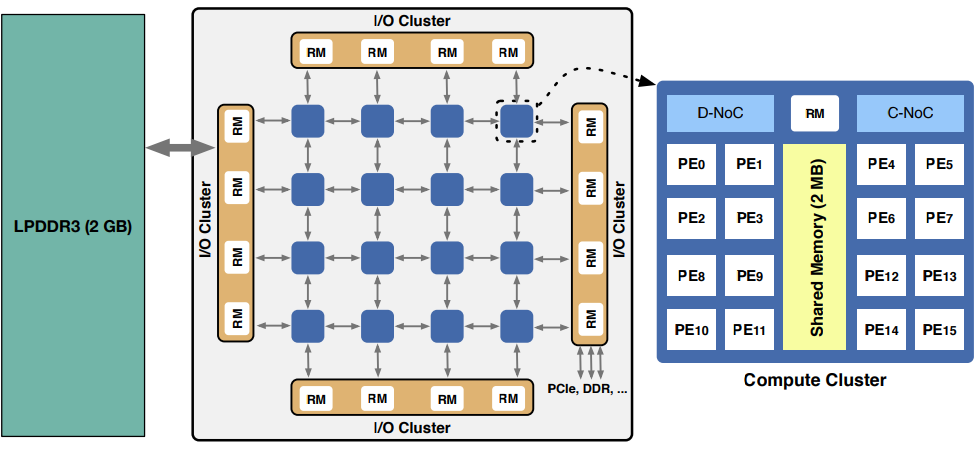
\includegraphics[width=0.7\textwidth]{figs/mppa.png} \\
		\end{tabular}
      \vspace{1ex} \\
      Fonte: (\citeonline{pskel:podesta})
     \end{center}
   \vspace{-2ex}
\end{figure}

%\end{figure}\includegraphics[width=10cm]{figs/25gray}

Além dos aspectos de hardware, aspectos de software também influenciam no desenvolvimento e, principalmente, no desempenho de aplicações para qualquer arquitetura.
O nível de abstração de hardware fornecido, assim como o sistema operacional utilizado, podem causar uma sobrecarga indesejada na execução de uma determinada aplicação \cite{Appel:1991:VMP:106972.106984, Cao:1994:IPA:1267638.1267651, Harty:1992:APM:143365.143511, Krueger:1993:TDA:165854.165867, Stonebraker:1981:OSS:358699.358703, Levy:Exception}.
Como solução, Engler \textit{et al}, propõe um pequeno \textit{kernel} que exporta, com segurança, todos os recursos de hardware através de uma interface de baixo nível.
Desta forma, bibliotecas e aplicações utilizam essa interface para implementar suas próprias abstrações, personalizando-as de acordo com o domínio da aplicação.
A separação entre proteção de recursos e gerenciamento permite a personalização específica das abstrações tradicionais de sistemas operacionais, estendendo, especializando ou até mesmo substituindo-as \cite{engler_exokernel:_1995}.

Neste contexto, a pilha de software disponibilizada pelo processador \mppa possui (i) suporte a programação paralela e distribuída, como \textit{POSIX}, \textit{OpenMP} etc; (ii) primitivas para sincronização e comunicação inter-processos (\ipc), tais como, \textit{sync}, \textit{portal} e \textit{mailbox}; e (iii) sistemas operacionais para cada tipo de \textit{cluster} como pode ser visto na figura \ref{figruntime}.
Nos \textit{Io Clusters}, é possível executar uma variação do sistema operacional Linux, \rtems, possibilitando a comunicação da máquina \textit{host} com o dispositivo, além da comunicação entre os \textit{IO} e \textit{Compute Clusters}.
Por outro lado, nos \textit{Compute Clusters}, o sistema operacional projetado para adequar-se aos 2-MB de memória local, \nodeos, é executado no \rman com o objetivo de auxiliar e gerenciar a comunicação dos \pe com os demais elementos do processador.


% FOTO DA SOFTWARE STACK
\begin{figure}[t]
	\begin{center}
    	\caption{Ambiente de execução do processador \mppa.}
           \label{figruntime}
		\begin{tabular}{ccc}
			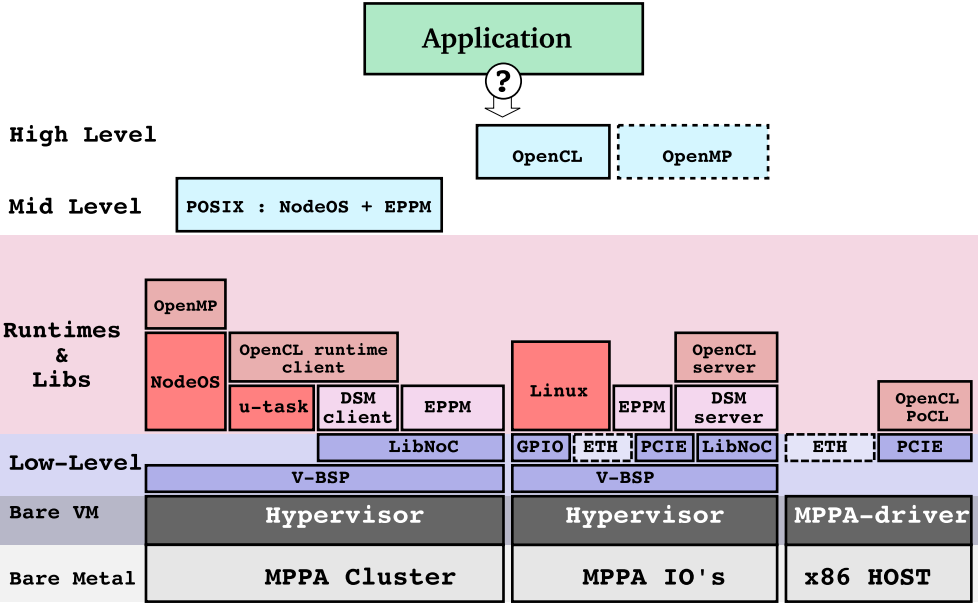
\includegraphics[width=0.7\textwidth]{figs/software_stack.png} \\
		\end{tabular}
      \vspace{1ex} \\
      Fonte: Documentação do processador \mppa
     \end{center}
   \vspace{-2ex}
\end{figure}

%\end{figure}\includegraphics[width=10cm]{figs/25gray}

Porém, ao utilizar esses \textit{runtimes} e abstrações de alto nível, uma aplicação estará acumulando a sobrecarga inserida pela pilha de software e as decisões de \textit{design} escolhidas no planejamento do ambiente de execução da Kalray.
Mesmo que a aplicação utilize adequadamente todos recursos disponíveis, ela deixará de explorar possíveis otimizações do seu domínio por não possuir acesso direto ao recursos do hardware.
Apesar disso, a Kalray também oferece bibliotecas de baixo nível com acesso direto aos recursos do processador, como a \textit{LibNoc} utilizada para \ipc.
% Embora a execução ainda aconteça sobre o \textit{hypervisor}, as camadas intermediárias são eliminadas, ... .
Contudo, essa opção aumenta o custo e complexidade do desenvolvimento das aplicações.

Uma alternativa viável, capaz de fornecer o gerenciamento e proteção dos recursos do processador \mppa, é o desenvolvimento de um \textit{exokernel} minimalista que utilize as bibliotecas de baixo nível disponíveis para prover uma camada de abstração de hardware (HAL)
% , com foco em fornecer primitivas \ipc,
que seja independente de plataforma.
Deste modo, os custos e complexidades no desenvolvimento vão ser amenizados pela maior familiaridade provida pelo \textit{exokernel} e portabilidade das aplicações permitindo o uso personalizado dos recursos disponíveis.

% Um exemplo de arquitetura \textit{manycore} é o processador \mppa  \cite{(CASTRO et al., 2013) emmanuel - proposta}, como pode ser visto na figure{mppa}, o \mppa é composto por 4 subsistemas de E/S, 16 clusters de computação e uma \noc responsável pela interconeção desses elementos.
% Cada subsistema de E/S possui 4 núcleos, compartilham uma cache coerente de 2 níveis e são responsáveis por realizarem a comunicação com a máquina \textit{host}.
% Cada \textit{clusters} de computação possui 16 núcleos de propósito geral, denominado \pe, 1 núcleo dedicado ao sistema operacional, denominado \rman, e compartilham 2-MB de memória local sem suporte à coerência de cache.
% A comunicação pode ser realizada através de duas \nocs distintas, uma de baixa banda para pequenas mensagens, denominada \cnoc; e outra com banda maior dedicada a transferência de dados, denominada \dnoc.


% % Exokernel approach
% Falar da camada exokernel, não implementa servições apenas expoe componentes de hardware para melhor gerenciamento

% % MPPA specs
% Arquitetura foco deste trabalho: Hardware e software

% % Problem Definition e justificativa
% Falar como pretendo usar bibliotecas de mais baixo nível para melhorar a performance e gargalo do SO para as aplicações

% % Results
% Uma abstração que forneça e gerencia recursos e que otimize o uso de tais recursos. Menos overhead do OS.

% Recentemente, vários processadores \textit{manycore} de alto desempenho e baixo consumo de energia estão surgindo. Um exemplo deles é o MPPA-256 \cite{Castro-IA3:2013}, que fornece um grande poder de processamento para o paralelismo de dados e tarefas com um baixo consumo de energia. Apesar desses processadores \textit{manycore} fornecerem uma melhor eficiência energética~\cite{Castro-IA3-JPDC:2014}, eles possuem uma arquitetura particular que torna o desenvolvimento de aplicações paralelas uma tarefa desafiadora~\cite{Varghese14,Castro-PARCO:2016,Castro-SBAC-PAD:2014}. Núcleos de processamento sem coerência de \textit{cache} são, geralmente, distribuídos em uma arquitetura organizada em \textit{clusters}, onde cada \textit{cluster} possui uma memória local (compartilhada somente entre os núcleos do \textit{cluster}). Dessa forma, a comunicação entre \textit{clusters} deve que ser efetuada através de uma Rede-em-Chip (\textit{Network-On-Chip} -- NoC) de maneira distribuída.
% Por essa razão, o tempo de comunicação pode variar entre os núcleos que estão se comunicando.
% %Explicar as dificuldades.

\section{Objetivos}

Utilizando os conceitos apresentados na seção anterior como base, o objetivo do TCC é desenvolver um \textit{exokernel} minimalista que exponha e proteja os recursos do processador \mppa.
Essa camada de abstração de hardware deverá  ser independente de plataforma, com o intuito de fornecer uma maior facilidade e menor custo no desenvolvimento das aplicações e bibliotecas que executam acima do \textit{exokernel}, sem a perda de desempenho ou do uso personalizado dos recursos.

O \textit{exokernel} deverá, dada a utilização das primitivas \ipc para comunicação e sincronização entre processos em \textit{clusters} distintos, realizar a alocação, proteção e multiplexação dos recursos necessários, além da configuração e envio/recebimento de dados.
Ao prover a comunicação, o \textit{exokernel} deverá implementar uma política de troca de mensagens assíncronas abaixo de sua interface, a fim de providenciar uma comunicação eficiente.
Para isso, o orientando necessitará utilizar as bibliotecas de baixo nível do processador \mppa. 

\begin{flushleft}
\textbf{Restrições:}
\begin{itemize}
\item Aplicações executadas no processador;
\item Utilizar a API do próprio processador;
\item Utilizar no máximo 2MB de memória nos \textit{clusters} do processador;
\item Utilizar no máximo 2GB de memória no sistema de entrada e saída.
\end{itemize}

\textbf{Premissas:}
\begin{itemize}
\item Processador disponível; 
\item Acesso ao processador de forma móvel; 
\item Computador disponível; 
\item Disponibilidade de Água; 
\item Disponibilidade de Luz; 
\item Disponibilidade de Energia; 
\item Acesso à Internet.
\end{itemize}

\textbf{Marcos:}
\begin{itemize}
\item Entrega da proposta: 08-05-2017; 
\item Entrega do projeto em fase inicial : 12-06-2017; 
\item Entrega do resumo em TCC I: 16ª semana de 17.2; 
\item Primeira entrega da monografia em TCCII: 9ª semana de 18.1; 
\item Apresentação da monografia: 13ª a 14ª semana de 18.1;
\item Segunda entrega da monografia em TCCII (versão final): 15ª semana de 18.1.

\end{itemize}
\textbf{Critérios de aceite:}
\begin{itemize}
\item Aprovação pela banca;
\item Aprovação do orientador;
\item Conformidade com as normas definidas pela instituição;
\item Prazos cumpridos;
\item Entregas cumpridas.
\end{itemize}
\end{flushleft}

Deve responder às perguntas: Como o trabalho será feito? Onde o trabalho será feito?
Com que ferramentas e meios o trabalho será feito?
Neste capítulo você mostrará como será executada a pesquisa e o desenho
metodológico que se pretende adotar: será do tipo quantitativa, qualitativa, descritiva,
explicativa ou exploratória.
Indique os passos de desenvolvimento do modelo ou produto se o TCC direcionado
para tal finalidade. A denominação Método de Pesquisa poderia ser substituída por
Procedimentos Metodológicos ou Materiais e Métodos.

\section{Método de Pesquisa}
 O andamento deste projeto ocorrerá em paralelo a pesquisa de doutorado do coorientador deste projeto, Pedro Henrique Penna, e utilizará como base o protótipo do sistema operacional \textit{multikernel} implementando pelo grupo de pesquisa Nanvix \cite{Penna2017,Penna2017-1} disponibilizado em \url{https://github.com/nanvix/multikernel}.

O desenvolvimento do trabalho será feito na linguagem C e dividido em cinco módulos, os quais são,
(i) \textbf{\noc Driver}: utilização da biblioteca de baixo nível da \noc para controle, manipulação e multiplexação dos \textit{buffers} de comunicação;
(ii) \textbf{Core Driver}: identificação e configuração dos elementos ativos do sistemas (\textit{IO e Compute Clusters}); 
(iii) \textbf{Sync}: abstração para sincronização entre processos localizados em \textit{clusters} distintos;
(iv) \textbf{Mailbox}: abstração para troca de mensagens pequenas, geralmente associadas a controle; e 
(v) \textbf{Portal}: abstração dedicada a troca de dados intensa. Os módulos \textit{sync} e \textit{mailbox} são dependentes dos primeiros módulos, assim como o \textit{portal} é dependente dos demais.

Os módulos e testes desenvolvidos utilizaram as bibliotecas e documentação disponibilizados pela Kalray e executados no processador MPPA-256, acesso remotamente em um servidor na França. O trabalho será efetuado no laboratório LaPeSD, localizado na Universidade Federal de Santa Catarina (UFSC), no qual o orientando possuirá acesso e uma máquina disponível para o desenvolvimento do trabalho. Além disso, o desenvolvimento deste trabalho ocorrerá associado a bolsa de iniciação científica do orientando, contribuindo com a sua formação e a qualidade final do trabalho desenvolvido.

% ----------------------------------------------------------
% PARTE - preparação da pesquisa
% ----------------------------------------------------------
% \part{Preparação da pesquisa}

% ----------------------------------------------------------
% Capitulo com exemplos de comandos inseridos de arquivo externo 
% ----------------------------------------------------------

\include{abntex2-modelo-include-comandos}

% ----------------------------------------------------------
% Parte de revisãod e literatura
% ----------------------------------------------------------
% \part{Revisão de Literatura}

% ---
% Capitulo de revisão de literatura
% ---
\chapter{Planejamento}

% ---
\section{Cronograma}

\newcommand{\cc}{\cellcolor{black!25}}  % Color cell
\arrayrulecolor{black}                  % Color lines

\begin{flushleft}
\begin{tabular}{|l|c|c|c|c|c|c|c|c|c|c|c|c|c|c|c|}
\hline
       & \multicolumn{8}{c|}{2017} & \multicolumn{7}{c|}{2018}\\ \hline
       
Etapas/Meses & 05 & 06 & 07 & 08 & 09 & 10 & 11 & 12 & 01 & 02 & 03 & 04 & 05 & 06 & 07 \\ \hline
%Fundamentação Teórica  & \cc & \cc & & &  &  &  &  &  &  &  &  &  &  & \\ \hline
%Estado da arte e prática  & & & \cc & \cc & & &  &  &  &  &  &  &  &  & \\ \hline
%Proposta da Solução  & & &  &  & \cc & \cc &  &  &  &  &  &  &  &  & \\ \hline
Desenvolv. da Solução  & \cc & \cc & \cc & \cc & \cc & \cc & \cc & \cc & \cc & \cc & &  &  &  & \\ \hline
Relatório Projeto I  & & &  &  &  &  & \cc & &  &  &  &  &  &  & \\ \hline
Conclusões  & & &  &  &  &  &  &  &  & \cc & \cc & &  &  & \\ \hline
Rascunho Projeto II  & & &  &  &  &  &  &  &  &  &  & \cc & &  & \\ \hline
Defesa  & & &  &  &  &  &  &  &  &  &  &  & \cc & & \\ \hline
Ajustes e Envio Final  & & &  &  &  &  &  &  &  &  &  &  & \cc & \cc & \cc \\ \hline
\end{tabular}
\end{flushleft}
% ---

% ---
\section{Recursos Humanos}

\begin{center}
\begin{tabular}{|c|c|}
\hline
    Papel & Nome \\ \hline
    Orientador & Márcio Bastos Castro \\ \hline
    Coordenador & Renato Cislaghi \\ \hline
    Membro da Banca I & Laércio Lima Pilla \\ \hline
    Membro da Banca II &  Mario Antônio Ribeiro Dantas\\ \hline
    Autor & João Vicente Souto \\ \hline
\end{tabular}
\end{center}
% ---

% ---
\section{Custos}

\begin{center}
\begin{tabular}{|c|c|c|c|c|c|}
\hline
\multicolumn{6}{|c|}{Estimativas para Recursos Humanos} \\ \hline
    Nome & Data Início & Data Fim & Hora/Mês & Valor/Hora & Custo Total \\ \hline
    Autor & 30/03/2017 & 29/06/2018 &  96 & R\$ 5,00 & R\$ 7200,00 \\ \hline
    Orientador & 30/03/2017 & 29/06/2018 & 8 & R\$ 65,00 & R\$ 7800,00 \\ \hline
    Coordenador & 10/11/2017 & 29/06/2018 & 1 & R\$ 137,00 & R\$ 959,00 \\ \hline
    Banca I & 10/11/2017 & 29/06/2018 & 1 & R\$ 65,00 & R\$ 455,00 \\ \hline
    Banca II & 10/11/2017 & 29/06/2018 & 1 & R\$ 135,00 & R\$ 945,00 \\ \hline
\multicolumn{5}{|l|}{Subtotal estimativas para recursos humanos} & R\$ 17359,00 \\
\hline
\end{tabular}
\end{center}

\begin{center}
\begin{tabular}{|c|c|c|c|c|c|}
\hline
\multicolumn{6}{|c|}{Estimativas para Recursos Não Humanos} \\ \hline
    Descrição & Data Início & Data Fim & Quantidade & Valor Unitário & Custo Total \\
    \hline
    CDs & 06/18 & 06/18 & 2 & R\$ 3,00 & R\$ 6,00 \\ \hline
    Impressão & 06/18 & 06/18 & 3 & R\$ 15,00 & R\$ 45,00 \\ \hline
\multicolumn{5}{|l|}{Subtotal estimativas para recursos não humanos} & R\$ 51,00 \\
\hline
\end{tabular}
\end{center}
% ---

% ---
\section{Comunicação}

\begin{center}
\begin{tabular}{|l|p{9cm}|}
\hline
    O que precisa ser comunicado & Entrega da Proposta \\ \hline
    Emissor & João Vicente Souto \\ \hline
    Receptor & Renato Cislaghi \\ \hline
    Comunicação & Será entregue a proposta completa do TCC \\ \hline
    Forma de comunicação & Sistema de TCC \\ \hline
    Frequência ou Quando & Única vez \\ \hline
\end{tabular}
\end{center}

\begin{center}
\begin{tabular}{|l|p{9cm}|}
\hline
    O que precisa ser comunicado & Entrega do Relatório em TCC I \\ \hline
    Emissor & João Vicente Souto \\ \hline
    Receptor & Renato Cislaghi \\ \hline
    Comunicação & Será entregue a primeira parte da monografia \\ \hline
    Forma de comunicação & Sistema de TCC \\ \hline
    Frequência ou Quando & Única vez \\ \hline
\end{tabular}
\end{center}

\begin{center}
\begin{tabular}{|l|p{9cm}|}
\hline
    O que precisa ser comunicado & Entrega da mografia completa em TCC II \\ \hline
    Emissor & João Vicente Souto \\ \hline
    Receptor & Renato Cislaghi \\ \hline
    Comunicação & Será entregue a monografia completa \\ \hline
    Forma de comunicação & Sistema de TCC \\ \hline
    Frequência ou Quando & Única vez \\ \hline
\end{tabular}
\end{center}

\begin{center}
\begin{tabular}{|l|p{9cm}|}
\hline
    O que precisa ser comunicado & Defesa do TCC \\ \hline
    Emissor & João Vicente Souto \\ \hline
    Receptor & Márcio Bastos Castro, Laércio Lima Pilla, Mario Antônio Ribeiro Dantas\\ \hline
    Comunicação & Será feita a defesa do TCC aos membros da banca.  \\ \hline
    Forma de comunicação & Pessoalmente \\ \hline
    Frequência ou Quando & Única vez \\ \hline
\end{tabular}
\end{center}

\begin{center}
\begin{tabular}{|l|p{9cm}|}
\hline
    O que precisa ser comunicado & Reuniões com o Orientador \\ \hline
    Emissor & João Vicente Souto \\ \hline
    Receptor & Márcio Bastos Castro \\ \hline
    Comunicação & Reuniões com o orientador para atualizações e dúvidas \\ \hline
    Forma de comunicação & Pessoalmente \\ \hline
    Frequência ou Quando & Quinzenalmente \\ \hline
\end{tabular}
\end{center}

\begin{center}
\begin{tabular}{|l|p{9cm}|}
\hline
    O que precisa ser comunicado & Enviar a monografia com ajustes após a defesa \\ \hline
    Emissor & João Vicente Souto \\ \hline
    Receptor & Renato Cislaghi \\ \hline
    Comunicação & Entrega da monografia com os ajustes necessários \\ \hline
    Forma de comunicação & Sistema de TCC \\ \hline
    Frequência ou Quando & Única vez \\ \hline
\end{tabular}
\end{center}
% ---

% ---
\newpage
\section{Riscos}

\begin{center}
\begin{tabular}{|l|c|c|c|c|l|}
\hline
    Nome & Probabilidade & Impacto & Exposição & 
    Estratégia & Ações de Prevenção  \\ \hline
    
     \makecell[l]{O acesso à máquina\\ está offline} & Média & Médio & Médio & Mitigar & - \\ \hline
     \makecell[l]{Computador não \\está mais funcionando} & Baixa & Médio & Média & Mitigar &\makecell[l]{ Tomar cuidado \\ ao manusear \\o computador e \\ não deixar bebidas \\ em lugares que \\ possam prejudicar \\ o computador.}  \\ \hline
     \makecell[l]{Outra pessoa está \\ utilizando a máquina \\ por um período longo} & Média & Médio & Média & Aceitar & -\\ \hline
     \makecell[l]{Orientador está\\ de viagem} & Média & Baixo & Médio & Mitigar & - \\ \hline
     \makecell[l]{Orientador fica doente} & Média & Baixo & Baixa & Mitigar & - \\ \hline
     \makecell[l]{Greve de ônibus} & Média & Baixo & Baixa & Mitigar & - \\ \hline
     \makecell[l]{O aluno ficou doente} & Média & Médio & Média & Aceitar & \makecell[l]{Fazer exercícios \\ e comer \\ regularmente \\ de forma \\ moderada e saudável.}\\ \hline
\end{tabular}
\end{center}
% ---


% ----------------------------------------------------------
% Resultados
% ----------------------------------------------------------
%\part{Resultados}

% ---
% primeiro capitulo de Resultados
% ---
%\chapter{Cap 2}

% ---
%\section{S}
% ---


% ---
% segundo capitulo de Resultados
% ---
%\chapter{Cap 3}

% ---
%\section{S}
% ---


% ---
% Finaliza a parte no bookmark do PDF, para que se inicie o bookmark na raiz
% ---
\bookmarksetup{startatroot}% 
% ---

% ---
% Conclusão
% ---
%\chapter*[Conclusão]{Conclusão}
%\addcontentsline{toc}{chapter}{Conclusão}

%\lipsum[31-33]

% ----------------------------------------------------------
% ELEMENTOS PÓS-TEXTUAIS
% ----------------------------------------------------------
\postextual

% ----------------------------------------------------------
% Referências bibliográficas
% ----------------------------------------------------------
\bibliography{bibliography}

% ----------------------------------------------------------
% Glossário
% ----------------------------------------------------------
%
% Consulte o manual da classe abntex2 para orientações sobre o glossário.
%
%\glossary

% ----------------------------------------------------------
% Apêndices
% ----------------------------------------------------------

% ---
% Inicia os apêndices
% ---
%\begin{apendicesenv}

% Imprime uma página indicando o início dos apêndices
%\partapendices

% ----------------------------------------------------------
%\chapter{Quisque libero justo}
% ----------------------------------------------------------

%\lipsum[50]

% ----------------------------------------------------------
%\chapter{Nullam elementum urna vel imperdiet sodales elit ipsum pharetra ligula
%ac pretium ante justo a nulla curabitur tristique arcu eu metus}
% ----------------------------------------------------------
%\lipsum[55-57]

%\end{apendicesenv}
% ---


% ----------------------------------------------------------
% Anexos
% ----------------------------------------------------------

% ---
% Inicia os anexos
% ---
%\begin{anexosenv}

% Imprime uma página indicando o início dos anexos
%\partanexos

% ---
%\chapter{Morbi ultrices rutrum lorem.}
% ---
%\lipsum[30]

% ---
%\chapter{Cras non urna sed feugiat cum sociis natoque penatibus et magnis dis
%parturient montes nascetur ridiculus mus}
% ---

%\lipsum[31]

% ---
%\chapter{Fusce facilisis lacinia dui}
% ---

%\lipsum[32]

%\end{anexosenv}

%---------------------------------------------------------------------
% INDICE REMISSIVO
%---------------------------------------------------------------------

%\printindex

\end{document}
